\documentclass{llncs}

\usepackage{subcaption}
\usepackage{subfig} 
\usepackage{usual}
\usepackage{graphicx}
\usepackage[noend]{algpseudocode}
\usepackage{subcaption}
\usepackage{subfig} 
\pagestyle{plain}

%
\begin{document}
\title{Agent utterances in dialogue of cooperative negotiation}
\maketitle 

For each utterance chosen by the user, we designed a tree of all the possible responses. These responses take in account the principals of dominance that we aim to model and the current state of the negotiation.

\section{State Preference (less,more)}
When the user states a preference that we note StatePreference(less,more), where $less, more \in C$.  We modeled the tree of choices, where each branch depends on the satisfiability of an applicability condition. Each branch of the trees is explained bellow:
	\begin{figure}[]
						\centerline{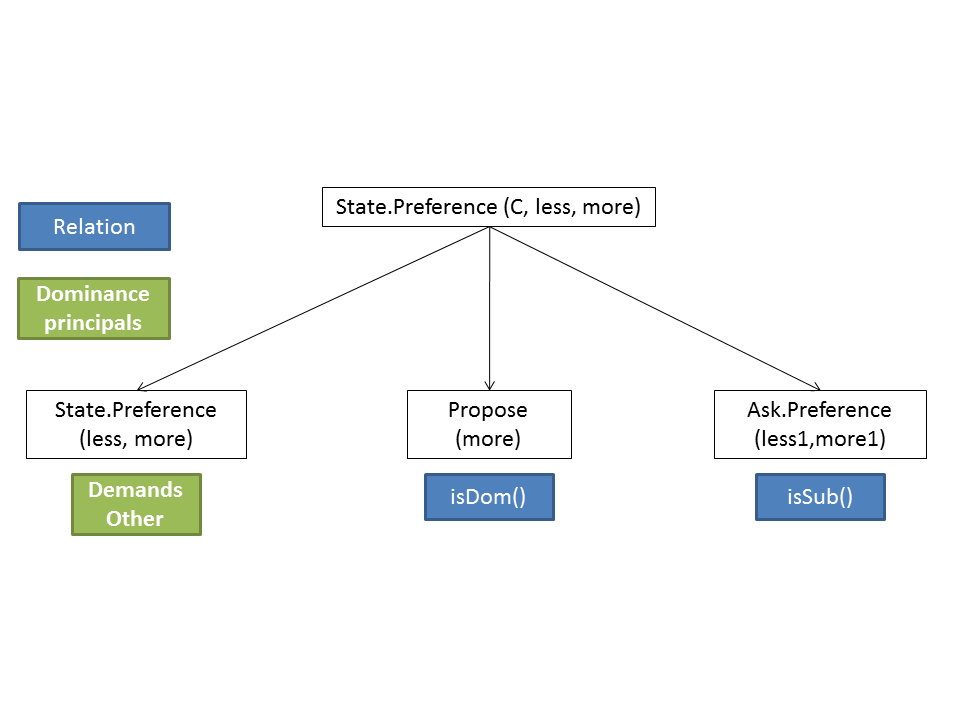
\includegraphics[width=3in]{figs/utterances_v2/Diapositive1.PNG}}
						\vskip 8pt
						\defig{state}{Tree of agent possible responses for a statePreference input.}
	\end{figure}
		
\begin{itemize}
	\item \textbf{Propose(C,More):} The agent proposes the preferred value. A propose is made only if the value is \emph{acceptable} for the agent. However, the value of acceptability varies depending on the relation of dominance. 
	\par  The acceptability of a value is computed with a function (see \fig{pseudo}) that considers the relation of dominance. First, dominant agent is very demanding, while the submissive one is not. Second, the submissive considers the preferences of the user. Indeed, if the user proposes a value that the agent already stated as not preferred, the agent will avoid a conflicting situation and accepts the value. The function isAcceptable(value, relation) is defined as follow: 
		\begin{figure}[]
			\begin{algorithmic}[1]\small
				\Function{isAcceptable}{$value$, $relation$}
					
					\If{($relation = dominant$)} 
						\State return $(score(value)> bestScoreOfPreference \times 0.7)$
					\EndIf
					\If{($relation = peer$)} 
						\State return $(score(value)> 0)$
					\EndIf
					\If{($relation = sub$)} 
						\State return $(score(value)> 0$  or $isInOAS(value))$
					\EndIf
				\EndFunction
			\end{algorithmic}
			\vskip 8pt
			\defig{pseudo}{Function to compute the acceptability of a value of preference}
		\end{figure} 
		
	\item \textbf{StatePreference(less',more')} : the agent reacts to the stated preference expressed by the user
	
			\begin{figure}[h]
					\begin{algorithmic}[1]\small
						\Function{reactToUser}{$less$, $more$}
							
							\If{($more = MostPrefferedValue()$ and $ (*, more) \notin OAS$)} 
								\State return $(*, more)$
							\EndIf
							\If{($more = LeastPrefferedValue()$ and $ (more, *) \notin OAS$)} 
								\State return $(more, *) $
							\EndIf
							\State The conditions $(2,4)$ are also applied for $less$
							\State $(less',more') = computePreference(less,more)$
							\If {$(less',more') \in OAS$}
								\State $(less1,more1)= reactToCriterion(more)$
								\If {$(less1,more1)=null$}
									\State $(less2,more2)= reactToCriterion(less)$
										\If{ $(less2,more2)=null$}
											\State return $(less',more')$
											\Else  
												return $(less2,more2)$
										\EndIf
								\EndIf
							\EndIf
							\State return $(less', more')$
						\EndFunction

					\end{algorithmic}
					\vskip 8pt
					\defig{react}{Function to react to a preference (less,more)}
				\end{figure}
		
		\item \textbf{AskPreference(less, more)}: I defined an AskPreference in the case of the submissive agent. However, when considering the structure of the tree, this branch is never executed. 

		
		
\end{itemize}
%

\section{AskPreference (less,more): } 
		When the user asks the agent about a preference, the agent calls the function reactToUser to compute a preference from the values of the askPreference.
		\begin{figure}[]
				\centerline{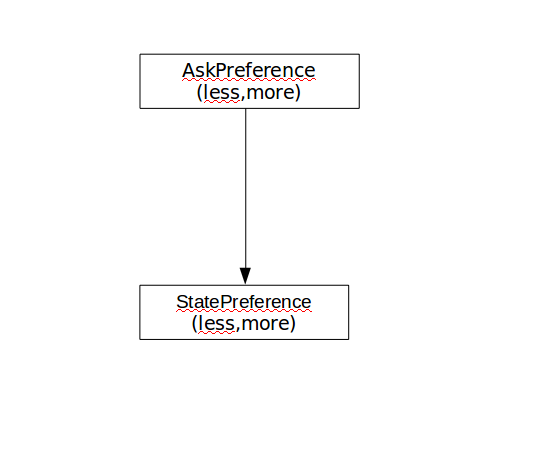
\includegraphics[width=3in]{figs/utterances_v2/askPref.png}}
				\vskip 8pt
				\defig{ask}{Tree of agent possible responses for an ask input.}
		\end{figure}
\section{Propose(proposal)}
	the user can either propose a value for a criterion or an option from the set of options of the topic of conversation. Thus, we define a proposal as a tuple $Proposal(Type, Value)$ where  $Type$ is either the the topic (for example Restaurants) or a criterion $c \in \mathcal{C}$ and value is:
	\begin{itemize}
		\item an option $O \in \in \mathcal{O}$ if $Type \in Topic$ 
		\item a value $v \in \emph{D}_c$ if $Type \in \mathcal{C}$
	\end{itemize}
	  \begin{figure}[]
	  						\centerline{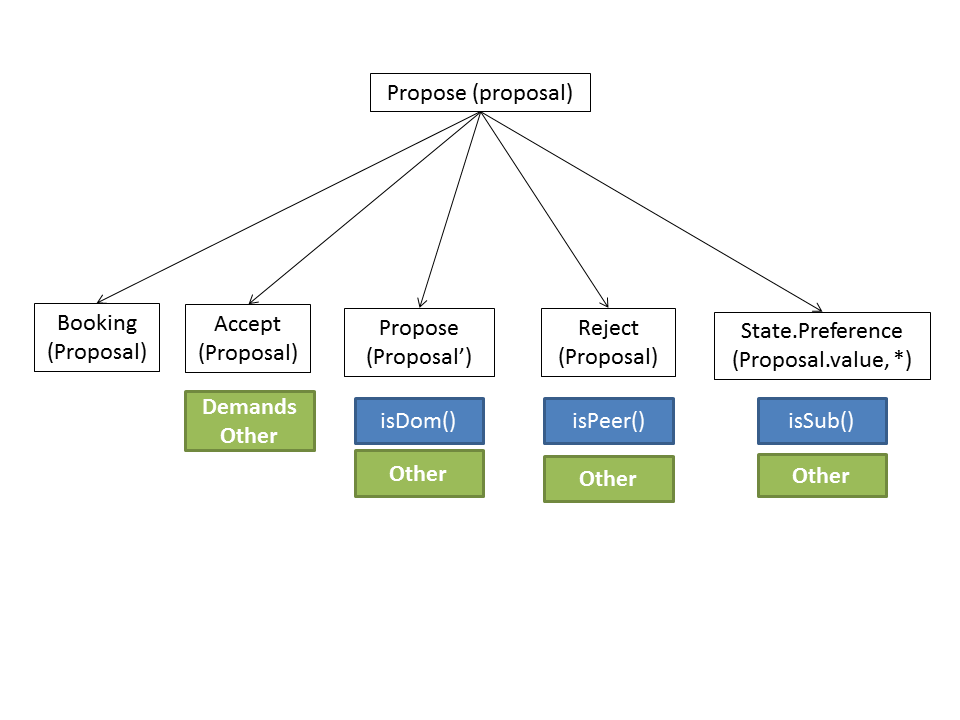
\includegraphics[width=3in]{figs/utterances_v2/Diapositive2.PNG}}
	  						\vskip 8pt
	  						\defig{prop}{Tree of agent possible responses for a propose input.}
	  	\end{figure}
\begin{itemize}
	\item \textbf{Booking:} In the case where a user proposes an option that is acceptable for the agent this later calls the task \textit{Booking}, to ask the user to book a table for the restaurant. 
	\item \textbf{Accept(Proposal):} the user proposes a value for a criterion that is acceptable for the agent. Thus, the agent expresses an accept.
	\item \textbf{Propose(Proposal'):} The user proposes a proposal which is not acceptable for the agent. This branch is applicable only if the agent is dominant in the relation. A dominant agent is demanding and self centered. Thus, if a user proposes a value which is not acceptable, the agent will counter propose with another value that better suits its preferences.
	\item \textbf{StatePreference(less,more):} The user proposes a proposal which is not acceptable for the agent, and the agent is submissive in its relation with the user. Instead of expressing a reject, the submissive agent will express a statement to express that the proposed value doesn't suit its preferences.
	In the case of an option, the agent computes the least scored value of this option to explain why he doesn't accept the proposal.
	\item\textbf{Reject(Proposal):} In the same case where the proposed value is not acceptable but the agent is not submissive to express his reject.
		
\end{itemize}

\section{Accept(proposal)}
\begin{figure}[]
		\centerline{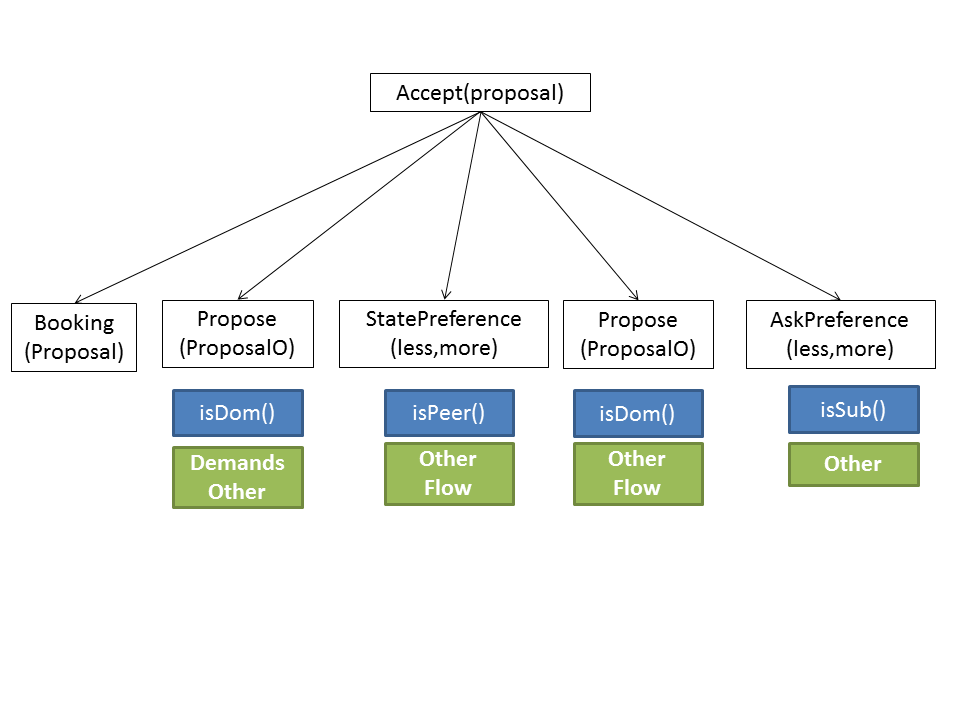
\includegraphics[width=3in]{figs/utterances_v2/Diapositive3.PNG}}
		\vskip 8pt
		\defig{accept}{Tree of agent possible responses for an Accept input.}
\end{figure}
\begin{itemize}
\item \textbf{Booking: } When the user accepts an option proposal , the agent closes the negotiation by proposing to book a table for the accepted restaurant (option).

\item \textbf{Propose(ProposalO):} when a user accepts a criterion proposal, a non-submissive agent continues the negotiation and proposes an option that is defined with the accepted value. However, a submissive agent will only propose an option, if the user accepts a value for each criterion of the topic.  The proposed option is defined with all the accepted values.
\item after accepting a value for a criterion, the agent opens a negotiation about another criterion of the topic to keep going on the negotiation. Wi distinguish three different responses with respect to the relation of dominance with the user:

	\subitem \textbf{StatePreference(less,more)}:  A peer agent opens a new subtopic or a negotiation on a criterion by expressing his preferences on this criterion.
	\subitem \textbf{AskPreference(less,more)}:  A submissive agent considers the preferences of the user and aims to satisfy them. Thus, to open a new negotiation on a criterion, he asks the user about his preferences on this criterion.
	\subitem \textbf{Propose(Proposal):} a dominant agent only considers his preferences. Thus, he directs the negotiation to satisfy them, by proposing his most preferred value on the new criterion. 
\end{itemize}
\section{Reject(proposal)}
	For the case of reject, we separate the responses depending on the value of the proposal(either a criterion or an option).
	\subsection{Reject(criterion)}
	\begin{itemize}
		\item \textbf{Propose(Proposal):} The rejected proposal value is the agent most preferred value for the discussed criterion, plus, the agent is dominant in its relation with the user. Thus, the dominant is demanding and self centered, he will keep proposing the proposal.
		\item \textbf{AskPreference(less,more):} When a submissive agent receives a reject, he assumes that his knowledge is not sufficient to negotiate. Therefore, he asks the user about his preferences on the current discussed negotiation. 
		\item \textbf{StatePreference(less,more):} A peer agent continues the negotiation by expressing his preferences on the current discussed criterion.
		\item\textbf{Propose(Proposal'):} A dominant agent leads the negotiation and keeps on proposing values on the discussed criterion.
		
	\end{itemize}
	\begin{figure}[]
			\centerline{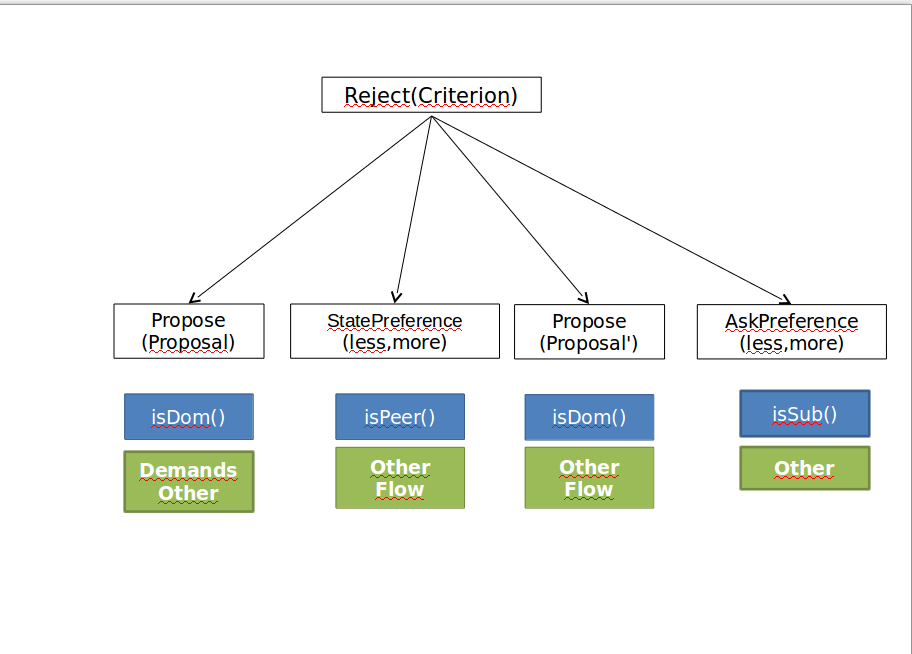
\includegraphics[width=3in]{figs/utterances_v2/RejectCrite.png}}
			\vskip 8pt
			\defig{rejectX}{Tree of agent possible responses for a reject criterion input.}
	\end{figure}
	
	\subsection{Reject(Option)}
\begin{itemize}
	\item \textbf{Propose(Proposal):} The rejected proposal value is the agent most preferred value for the discussed criterion, plus, the agent is dominant in its relation with the user. Thus, the dominant is demanding and self centered, he will keep proposing the proposal.

	\item \textbf{AskPreference(less,more)}: An option proposal is always proposed by the agent when at least a criterion proposal has been accepted. Therefore, if the user rejects an option proposal, means that the agent still ignores user preferences on the other criteria of the option. The submissive agent which is centered on the user preferences will try to gather more knowledge on the user preferences.

	\item \textbf{StatePreference(less,more)} : the peer agent follows the same behavior of gathering knowledge on preferences on other criteria. Therefore, he opens the negotiation by stating his preferences on the new discussed criterion. By consequence, the agent manages the flow of the negotiation. 
	
	\item \textbf{Propose(Proposal'):} when a non submissive agent receive a reject, he will want to continue the negotiation by proposing other proposals. The agent continue the negotiation by proposing other proposals, which represent the principal of controlling the flow of the conversation.
\end{itemize}
\begin{figure}[]
		\centerline{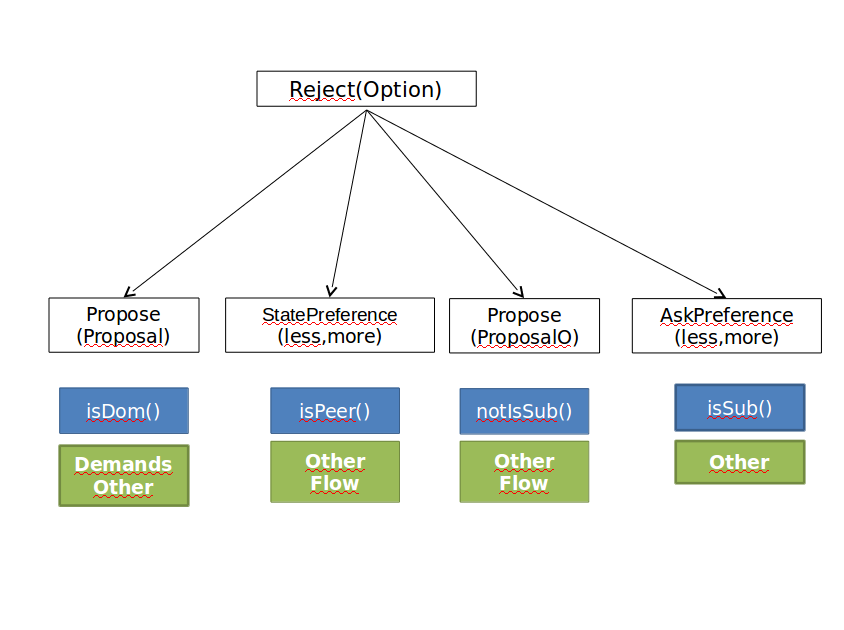
\includegraphics[width=3in]{figs/utterances_v2/RejectOption.png}}
		\vskip 8pt
		\defig{RejectO}{Tree of agent possible responses for a reject option input.}
\end{figure}

\textbf{Note:} Each produced tree is defined with an exit condition, that checks if the negotiation is at an dead end and there is no possible remaining compromise to find.
	Dominant case
	Submissive case:
\end{document}